%\documentclass[10pt,a4paper]{article}

\documentclass[24pt]{article}

\usepackage{arxiv}
\usepackage[utf8]{inputenc} % allow utf-8 input
\usepackage[T1]{fontenc}    % use 8-bit T1 fonts
\usepackage{hyperref}       % hyperlinks
\usepackage{url}            % simple URL typesetting
%\usepackage{booktabs}       % professional-quality tables
\usepackage{amsfonts}       % blackboard math symbols
\usepackage{nicefrac}       % compact symbols for 1/2, etc.
\usepackage{microtype}      % microtypography
\usepackage{lipsum}         % Can be removed after putting your text content
\usepackage{graphicx}
\usepackage{natbib}
\usepackage{doi}
\usepackage{amssymb}
\usepackage{amsthm}
\usepackage{forest}


\usepackage{tikz} 
\usepackage{caption}
\usepackage{amsmath}
\usepackage{cleveref}       % smart cross-referencing
\usepackage{colortbl}
\usepackage{color}
\usepackage{listings}
\usepackage{multicol}


\definecolor{orange151}{rgb}{0.9,0.647,0}
\definecolor{lgreen}{rgb}{0.564,0.93,0.564}


\usepackage{color}

\definecolor{dkgreen}{rgb}{0,0.6,0}
\definecolor{gray}{rgb}{0.5,0.5,0.5}
\definecolor{mauve}{rgb}{0.58,0,0.82}

\lstset{frame=none,
  language=Python,
  aboveskip=3mm,
  belowskip=3mm,
  showstringspaces=false,
  columns=flexible,
  basicstyle={\small\ttfamily},
  numbers=none,
  numberstyle=\tiny\color{gray},
  keywordstyle=\color{blue},
  commentstyle=\color{dkgreen},
  stringstyle=\color{mauve},
  breaklines=true,
  breakatwhitespace=true,
  tabsize=3
}
\definecolor{dgreen}{rgb}{0,0.5,0}
\definecolor{bg}{rgb}{0.125,0.51,0.49}
\definecolor{mag}{rgb}{0.866,0.627,0.866}
\definecolor{lgray}{rgb}{0.49,0.49,0.49}
\definecolor{dgray}{rgb}{0.82,0.788,0.827}
\definecolor{pink}{rgb}{1, 0.568, 0.686}
\definecolor{lblue}{rgb}{0.078, 0.741, 0.931}
\definecolor{orag2}{rgb}{0.87, 0.478, 0.12}

\newcommand*{\addheight}[2][.5ex]{%
  \raisebox{0pt}[\dimexpr\height+(#1)\relax]{#2}%
}

%\newcommand{\subf}[2]{%
%  {\small\begin{tabular}[t]{@{}c@{}}
%  #1\\#2
%  \end{tabular}}%
%}

\newtheorem{theorem}{Theorem}[section]
\newtheorem{lemma}[theorem]{Lemma}
\newtheorem{proposition}[theorem]{Proposition}
\newtheorem{corollary}[theorem]{Corollary}
\newtheorem{example}[theorem]{Example}
\newtheorem{definition}[theorem]{Definition}


\title{Elaborating pipelines for image analysis in the context of cell biology}

%\author{ \href{https://orcid.org/0000-0002-8749-3324}{
\includegraphics[scale=0.08]{orcid.pdf} \href{mailto: jacques.bourg739@gmail.com}{@}\hspace{1mm} Jacques Bourg    }}
\author{Jacques Bourg}


% Uncomment to override  the `A preprint' in the header
\renewcommand{\headeright}{}
\renewcommand{\undertitle}{}
\renewcommand{\shorttitle}{Pipelines for image analysis}


\hypersetup{
pdftitle={Elaborating pipelines for image analysis in the context of cell biology},
pdfsubject={math.NT},
pdfauthor={Jacques Bourg},
pdfkeywords={Python, image analysis, image processing, pipelines, cell biology, omics.},
}
 

\begin{document}

\maketitle

\begin{abstract}
  A routine experiment for a molecular biologist is to image cells in a specific medium and measure their response in presence of a particular stimulus. Often, this response is quantified using image analysis. 
In this white paper, I will detail the main steps involved in creating a pipeline for image analysis and quantification of RNA expression in cells. The main methodology for pipeline creation should remain valid across a series of cell structures and biological questions.
\end{abstract}

\keywords{Python, image analysis, image processing, pipelines, cell biology, omics.}

\section{Introduction}
 

\subsection{Biological context }

Measuring gene expression is very important in biology because it provides a dynamic snapshot of what's happening inside cells at a given time. It is an window into life's processes in both health and disease.
Using fluorescence imaging, we can measure the levels of rna expression. This technique is called FISH (fluorescence in situ hybridisation).  Briefly, oligos are designed to bind specifically to gene sequences, and these oligos are linked through other complementary molecules, to fluorophores, small fluorescent molecules that absorb light at a a given wavelength and emit back light at a higher wavelength. In one of the projects I participated in, our collaborators targeted HOX genes. These genes are involved in patterning the body plan of animals during embryonic development. Through image analysis, we could quantify the expression of two of them (HOXC8 and HOXA10) at different time points when stimulated with different growth differentiation factors (GDF-FDF, GDF and NT). 
 
\subsection{Experiment description} 
 
 An usual experiment goes like this: cultured cells are fixed on a microscope slide.  Then, a fluorescent probe (or a mixture of them) is applied to the cells. The probes hybridize in a complementary way to the target sequences of a gene of interest. There is then a first washing to remove excess and non-specifically bounded probes. Finally, the sample is visualized under a fluorescence microscope. Single dots 
 indicate the presence of a gene of interest. As shown in the schematic, a single fluorophore has a diameter smaller than 2 nm, and a usual image pixel is around 100 nm square. Nonetheless the difference in orders of magnitude, a single fluorophore can spread over some pixels, due to the microscope point spread function (PSF), which is due to light diffraction. The noise in these experiments arises from non-specific probe binding, from autofluorescence of certain structures, and from residual contamination from previous wash steps.
 
  
 
  \begin{figure}[h!] % Placement options: h=here, t=top, b=bottom, p=page, !=override
  \centering
  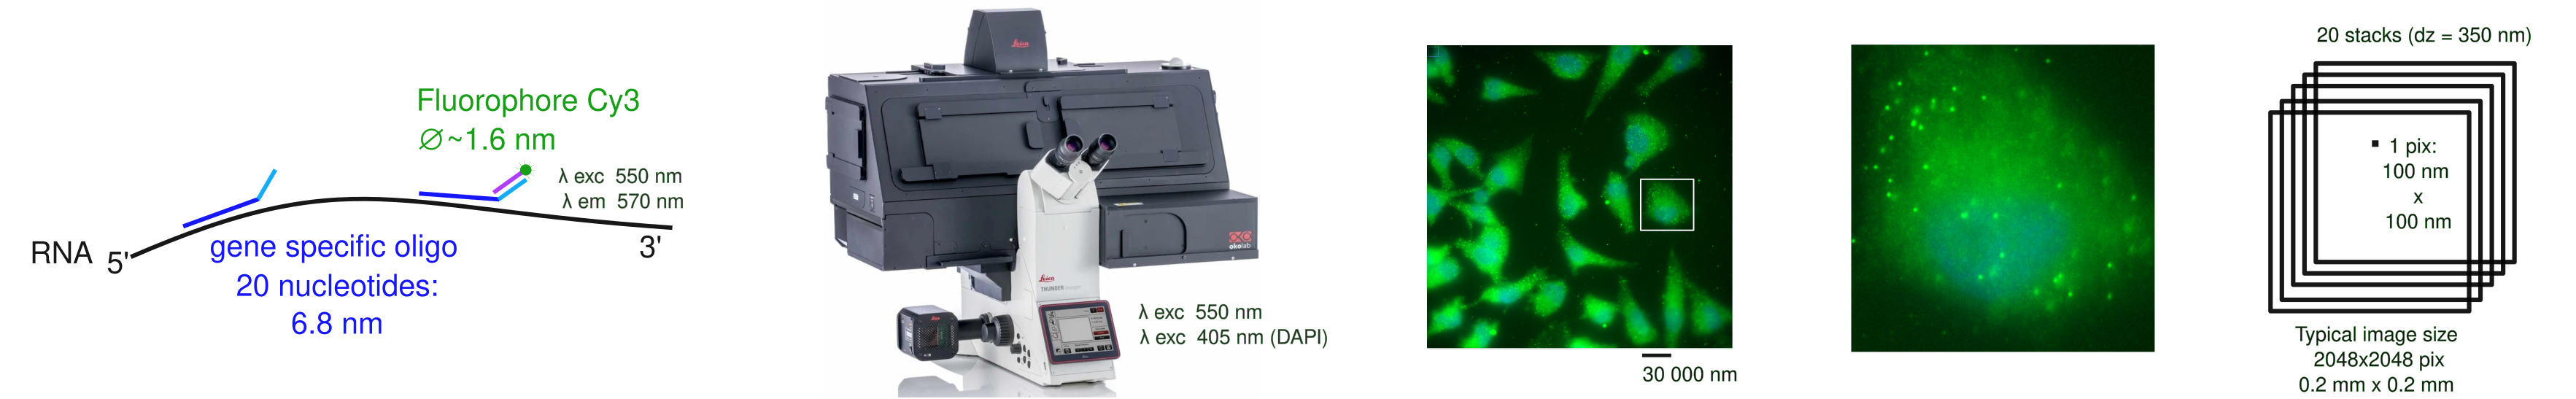
\includegraphics[width=1\textwidth]{Experiment_description.png} % Adjust width as needed
  \caption{Experiment description.}
  \label{fig:my_image} % For referencing the figure later
\end{figure}


  

 
 
 \newpage
\section{Pipeline construction} 
 
In the following I will detail how I built an analysis pipeline. I will first go over the main computation steps, to then focus on the aspects related to the implementation, for instance, aspects related to the folder architecture and data format. 
        
\subsection{Pipeline overview} 

 \begin{figure}[h!] % Placement options: h=here, t=top, b=bottom, p=page, !=override
  \centering
  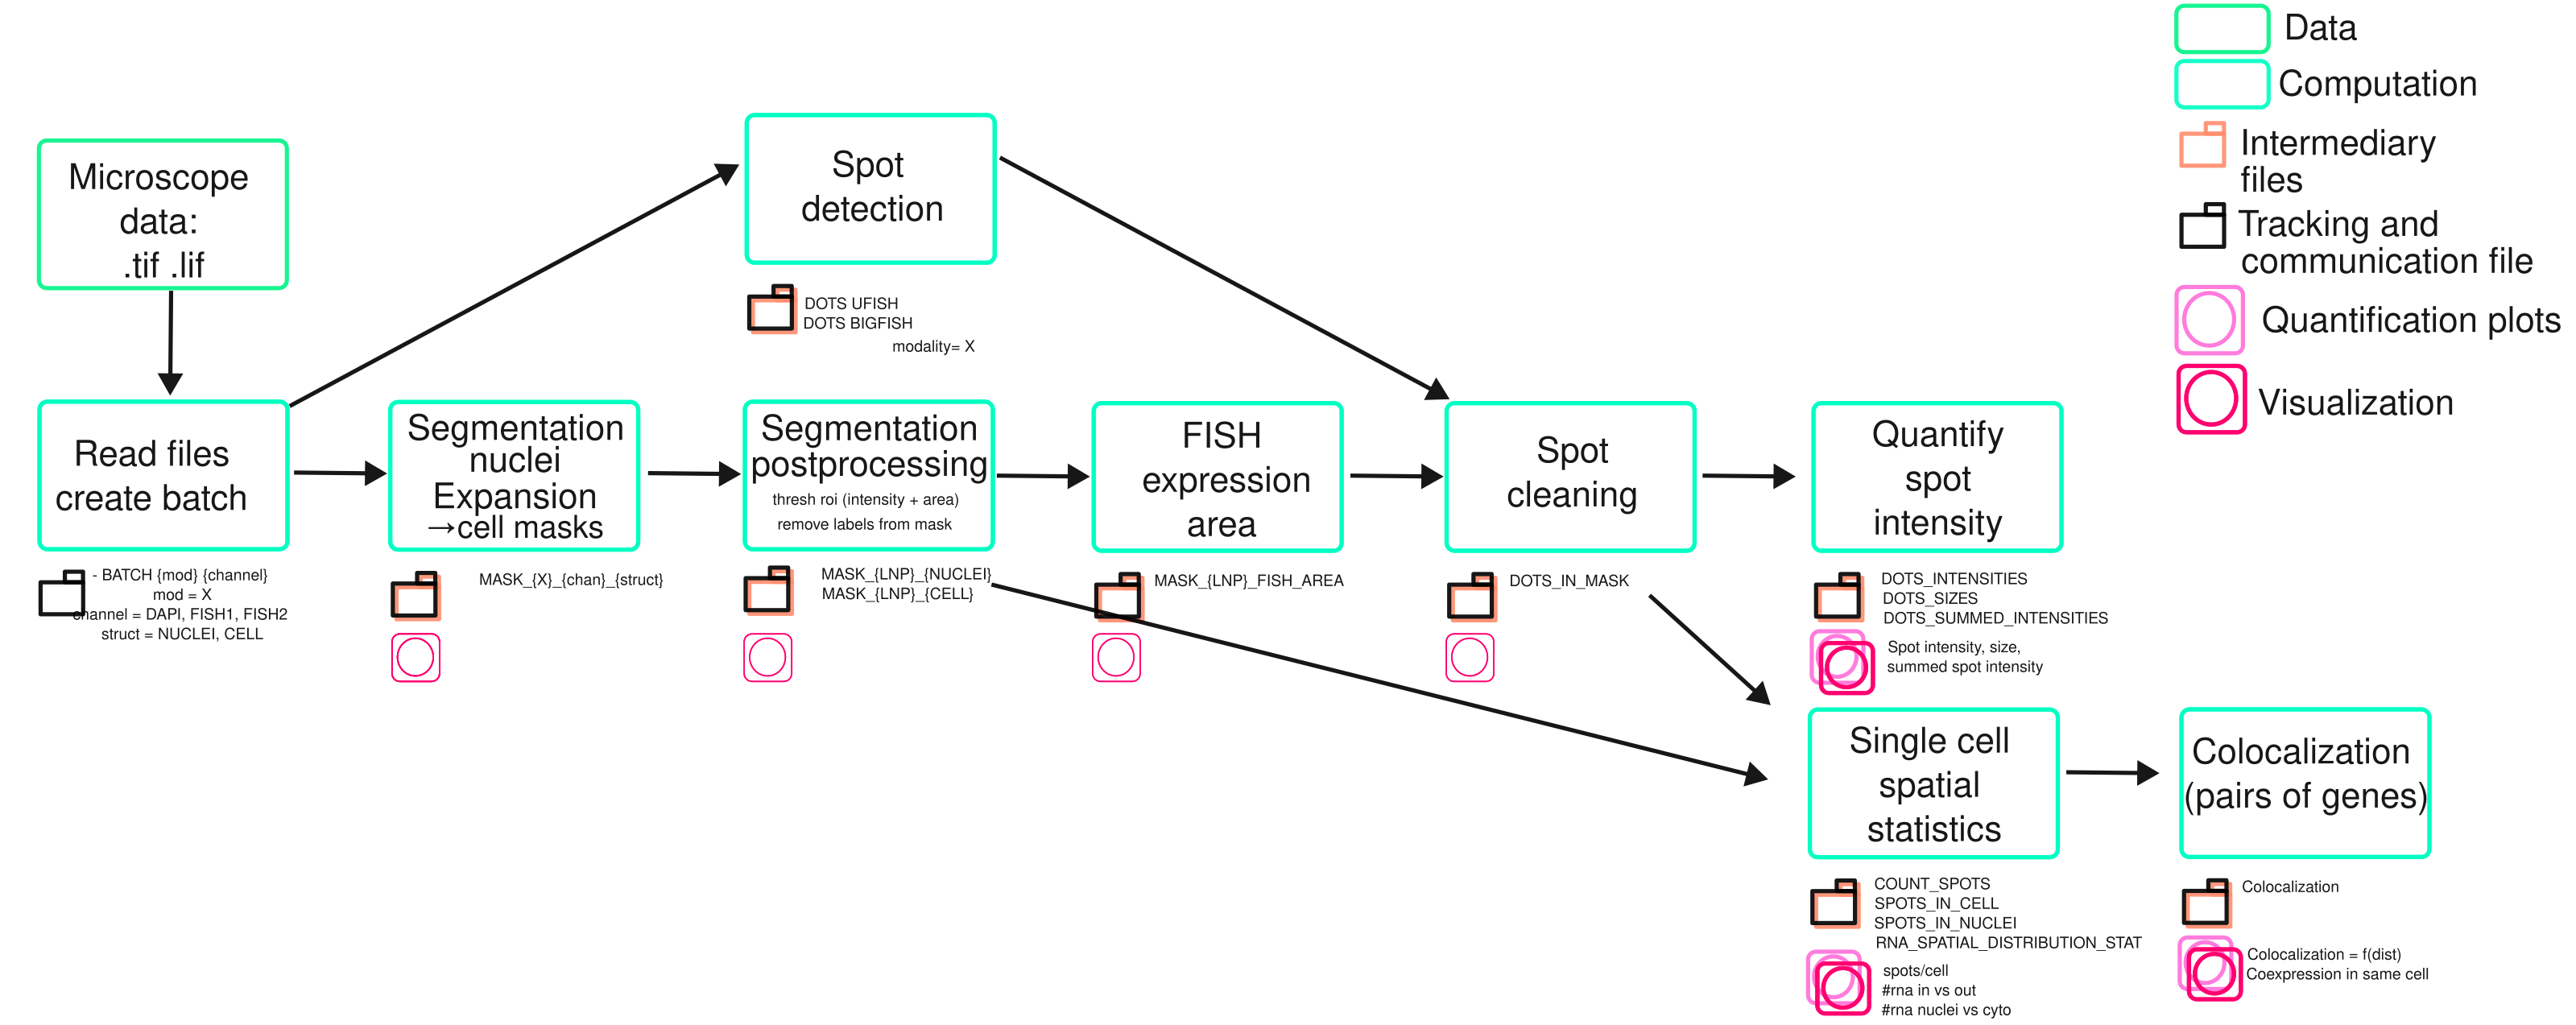
\includegraphics[width=1\textwidth]{HOX_pipeline.png} % Adjust width as needed
  \caption{Image analysis pipeline.}
  \label{fig:my_image} % For referencing the figure later
\end{figure}
 
  \newpage
 
\subsection{Main pipeline steps} 

\subsubsection{Segmentation and post-processing}
 
 We are interested in segmenting the nuclei and the cell membrane. Cells are densely packed into clusters, and the cytoplasm is invisible. I  trained Cellpose on the nuclei, and in order to account for the RNAs which are close to the nuclei, I did a small dilation of the cellpose masks (using watershed algorithm) and then deduced the cell masks. Those cellmasks are stored in the corresponding folder (see folder  structure).

We train two different models, one for nuclei and the other cell membrane.   Sometimes these two models, even well trained ones, might fail and for instance do not detect a cell,  but detect the  nuclei. In this case, we apply a postprocessing consisting in removing cell segmentations in which there is no nuclei segmentation inside of the cell or the converse. In the case of this particular pipeline, this never happens, since out of the detected nuclei, we deduce a mask for the cell body segmentation, and this mask has the same label number as the nuclei, but in many cases this has to be sorted. In the presented pipeline, we remove, using a napari app, putative nuclei with a small area, or very bright: these are either portions of nuclei off the focus or dying nuclei. Another common problem is that nuclei have to be inside the cells. In the case in which the segmentation mask  of the nuclei overfills the segmentation mask of the cell. In this case, the cell mask is updated taking the union of the two masks. 
 
 
\subsubsection{Spot detection and spot cleaning} 

There are two families of algorithms of spot detection, the ones based on signal processing and the ones based on deep learning. In this
pipeline I used two algorithms: BigFish \href{https://rnajournal.cshlp.org/content/28/6/786.long}{[BigFish]} and Ufish \href{https://www.biorxiv.org/content/10.1101/2024.03.06.583706v1.full.pdf}{[Ufish]}   from each of the two classes.
BigFish spot detection proceeds by convolving a Laplacian of Gaussians kernel with the image, inverting and rectifying it, and then detect the maxima and retaining only the maxima which are above a certain threshold. Out of this, we find the coordinates of these spots. 


 \begin{figure}[h!] % Placement options: h=here, t=top, b=bottom, p=page, !=override
  \centering
  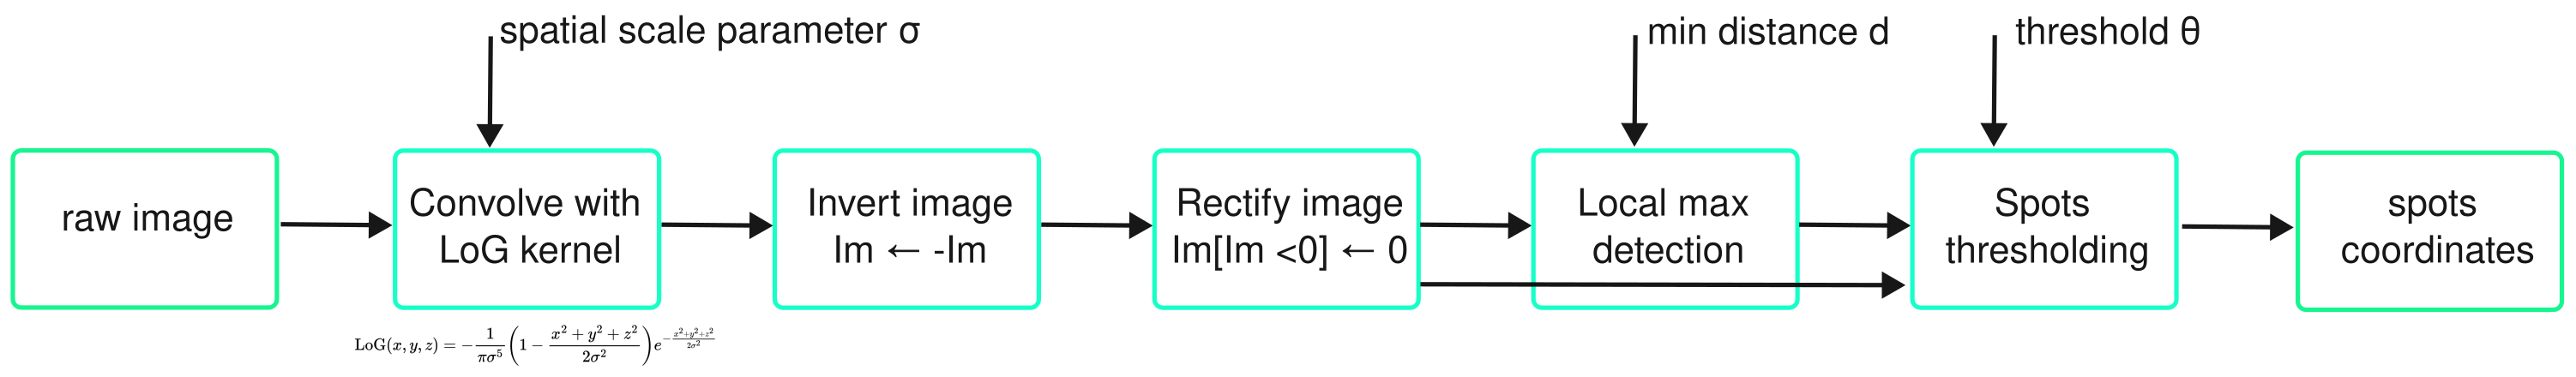
\includegraphics[width=1\textwidth]{BigFISH_pipeline.png} % Adjust width as needed
  \caption{Big Fish pipeline.}
  \label{fig:my_image} % For referencing the figure later
\end{figure}
Ufish uses rather a U-Net to  preprocess and enhance fish images.

 \begin{figure}[h!] % Placement options: h=here, t=top, b=bottom, p=page, !=override
  \centering
  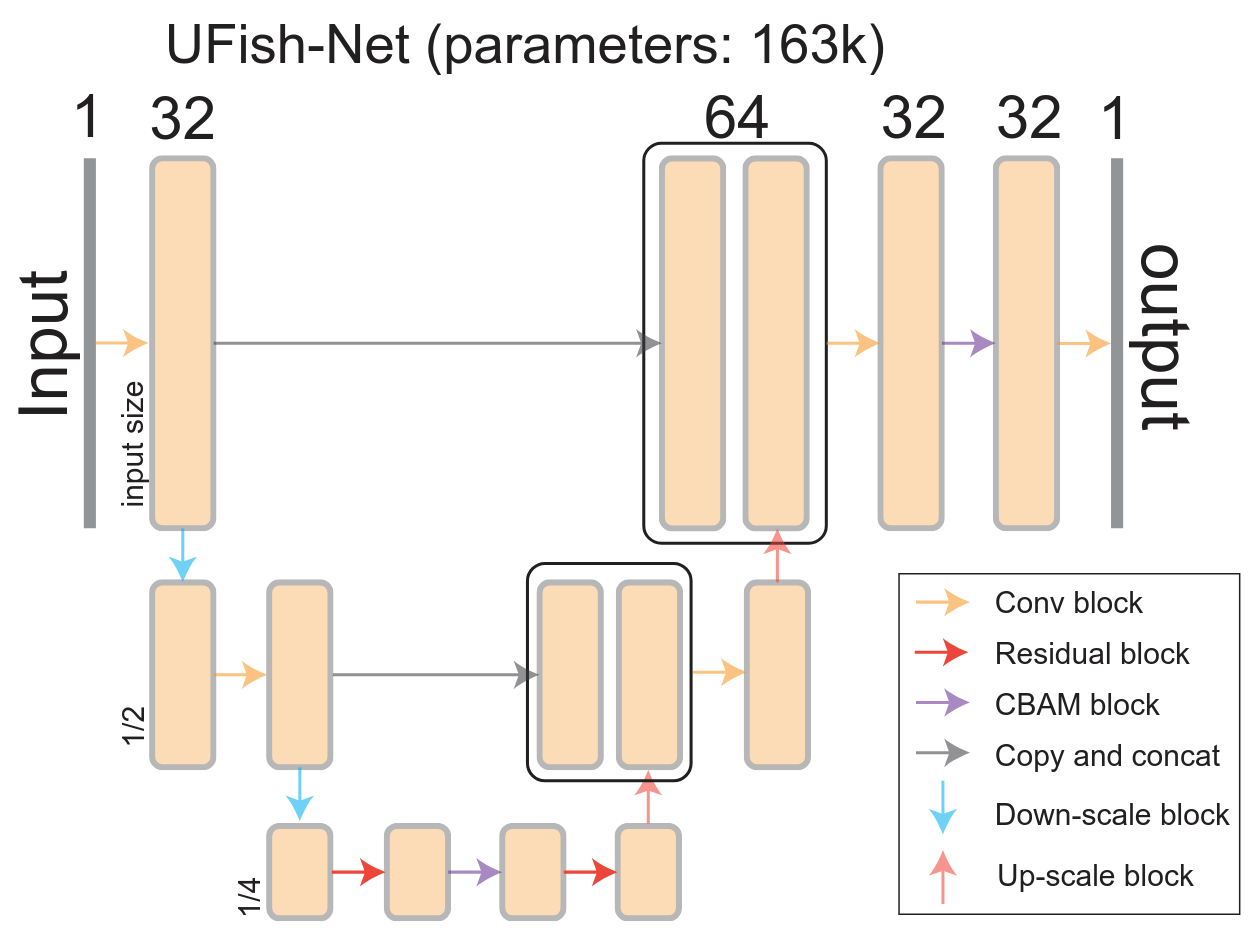
\includegraphics[width=0.3\textwidth]{ufish.png} % Adjust width as needed
  \caption{U FISH spot detector.}
  \label{fig:my_image} % For referencing the figure later
\end{figure}


Spot cleaning is about to retain only spots that are close to cells. To achieve this we compute a binary mask composed of all cell labels, and expand it using a dilation operation of a given length. In that way, only spots that are in that mask are retained. 


\subsubsection{Measure features and statistics} 

Once the spots are detected and the cell and the nuclei segmented, a certain number of measures can be taken, for instance the intensity of each spot or its signal-to-noise ratio. We can also visualize the distributions of these quantities or the single cell statistics, like the number of spots per cell, the count of spots in the nuclei and in the cytoplasm, and even characterize spatially the distribution of cells, using indexes like the polarization index, which quantifies the degree to which RNA molecules are non-uniformly distributed or concentrated in specific subcellular regions.


 
  
  \begin{figure}[h!!] % Placement options: h=here, t=top, b=bottom, p=page, !=override
  \centering
  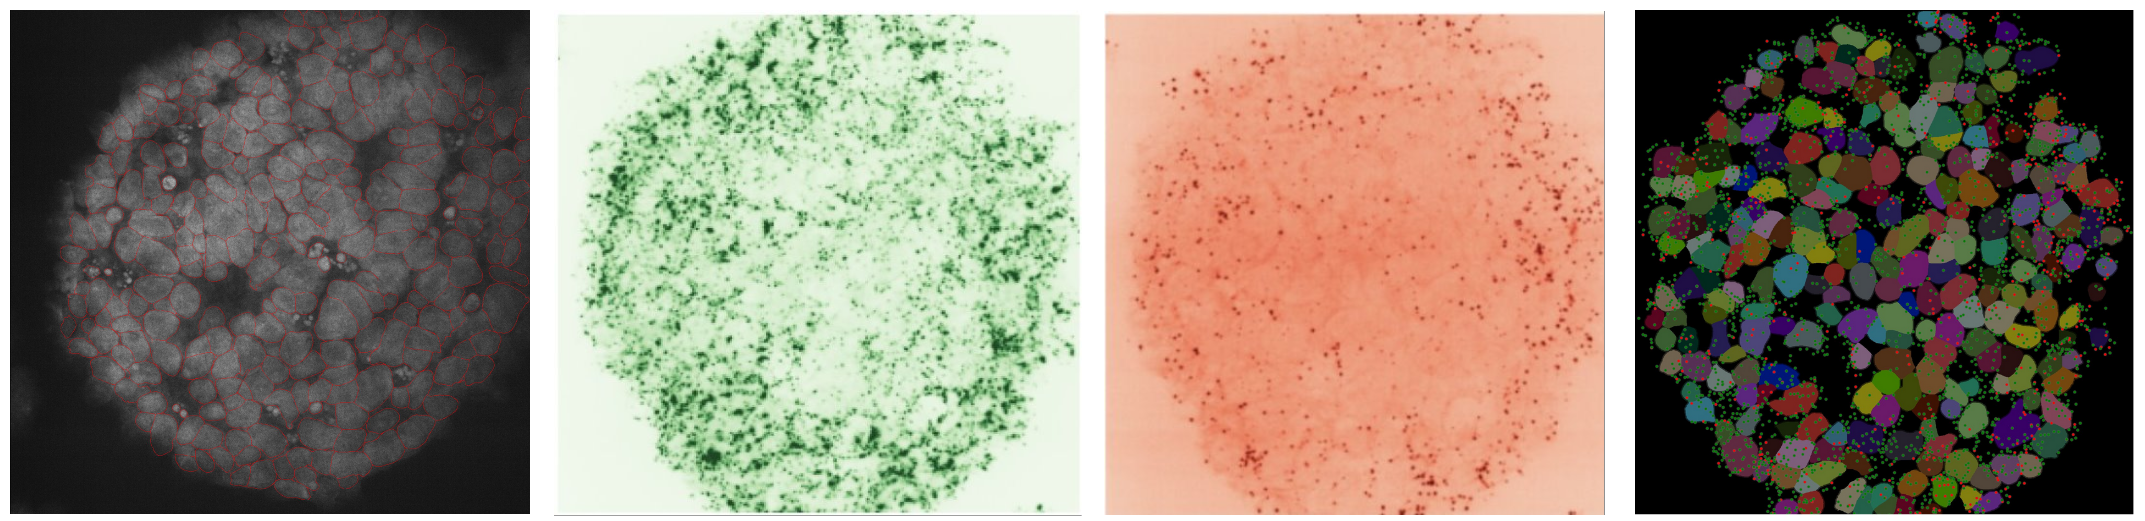
\includegraphics[width=.8\textwidth]{pipeline_raw_data_results.png} % Adjust width as needed
  \caption{Cell segmentation and spot detection.}
  \label{fig:Raw_data} % For referencing the figure later
\end{figure} 


 \newpage


\section{Pipeline construction}

\subsection{Intermediary file formats and data manipulation} 

To store the results, we followed the convention of  standarized fish omics formats \href{https://fish-omics-format.readthedocs.io/en/latest/intro.html}{[1]}.
The use of such standards is essential for data sharing, for reproducibility and for interoperability with other technologies. 


For each field of view / imaging session, we create a separate .csv file. In here I show a file with all the spots found.  Spots are detected with their coordinates (2D or 3D). Therefore, after spot detection, an unique spot identifier is assigned to each spot ($\text{Spot\_ID}$),  together with its coordinates.  This is fundamental for traceability and quality control along the pipeline. Further measures can add new columns, (for instance, measuring the intensity). For some spots we do not measure some properties, but it is due to the spot cleaning procedure. 

In order to be able to load and save the data in an easy way, I stored together with the .csv files a numpy file (.npy) containing a dictionary, with the addresses of all the csv files, in such a way that, though appropriate functions, I could charge in one line a dictionary with as keys the file names and as values, dataframes with all the information needed.

Example of header for spot format :


\begin{table}[h!]
    \centering
    \caption{Spot Data Table}
    \label{tab:cell_data}
    \begin{tabular}{|l|c|c|c|c|c|c|c|c|c|c|c|c|}
        \hline
        \textbf{Spot ID} & \textbf{Y} & \textbf{X} & \textbf{In mask} & \textbf{Int.} & \textbf{Width} &  \textbf{snr} &  \textbf{back.} &  \textbf{in cell} &  \textbf{cell mask} &\textbf{in nucl.} & \textbf{in cyto}      \\
        \hline
        1	& 641	&1748	& T	&2151 &	5.4	& 3.20 &	1807.18 &	T 	&3.0 &	0.0	&1.0 \\
        \hline

2		&1466	&1114	&T	&2198 &	1.3 &	3.38 &	1851.8 &T &	7.0 &	1.0 & 	0.0 \\
        \hline
3		&1507	&1663	&F	&  &	  &	 &	&		& 	& 	 & \\
        \hline        
    \end{tabular}
\end{table}






Example of header for single cell statistics:


\begin{table}[h!]
    \centering
    \caption{Cell Data Table}
    \label{tab:cell_data}
    \begin{tabular}{|l|c|c|c|c|c|c|}
        \hline
        \textbf{Cell ID} & \textbf{Counts} & \textbf{Count Nuclei} & \textbf{Count Cyto} & \textbf{Pol. Ind.} & \textbf{Disp. Ind.} & \textbf{Per. Dist. Ind.} \\
        \hline
         1 & 5 & 3 & 2 & 0.52 & 0.76 & 1 \\
         \hline
         2 & 13 & 4 & 9 & 0.31 & 1.12 & 1.1 \\
         \hline
         3 & 5 & 1 & 4 & 0.92 & 0.24 & 0.57 \\
        \hline
    \end{tabular}
\end{table}

 
 For cellmasks, we store them in .png files.

 
 
\subsection{Parameters tracking and communication between notebooks}

In the folder named Code, I put the Jupyter notebooks. Jupyter notebooks have to be run in a certain order, the order proposed in the pipeline overview. Also, in order to communicate between notebooks and to track all the important variables I save, as I execute the pipeline,  in a .json file all the variables that are necessary to reproduce the figures, and to communicate between notebooks. 

To do this, I name important variables in uppercase and then, at the end of the notebook, I store in a .json file all the variables that are written in uppercase with their respective values.   
 
 
 
 
\subsection{Code modularity}

         Notebooks like ‘Max projection’ may have to be run twice, one for the cell and one for the nucleus. This is due to the fact that in some experiments we use the DAPI channel to do the max projection that will be used to segment the nuclei. However, in order to segment the cell, it depends on the experiment. In some experiments, we use the fish channel (with the spots) to detect the cell membrane, which gives imperfect results, but it is the best we can do. Finally, in some experiments, 
we add to the DAPI, a substance called  'cell mask' that allows to stain the cytoplasm, and then to use only one channel for the nuclei and cell membrane detection.

The way we achieve code modularity is by defining constants at the beginning and through  the pipeline, loading them, and storing them in the .json file.  This also implies to create different 
folders to store the intermediary files.


The way to create for instance a new variable in uppercase with the right name is done using dynamic programming. For instance, in the first notebook, 'Read files create batch', I created a simple widget to enter the list of genes observed, for instance HOXC8 and HOXA10. These names are stored in the .json. When we load the .json file in another notebook as a dictionary that I call 'constants', the dictionary key CHANNELS contains two values with the gene's names: HOXC8 and HOXA10.


A user can then choose manually, through  Dropdown widgets, the variable $ \text{chan\_f}$ that will contain the value, HOXC8 for instance. 

In order to load the max projection of the corresponding 3D image with the gene HOXC8, I call the variable, using f-strings:


$$ \text{batch\_fish\_mip} = \text{constants[f'BATCH\_\{\text{modality}\}\_\{\text{chan\_f}\}\_\{\text{struc\_cell}\}\_MIP']} $$
 

 
 
%
%For cellmasks, we stored them in .png files.
\newpage

\subsection{Folder structure}

 \begin{figure}[h!] % Placement options: h=here, t=top, b=bottom, p=page, !=override
  \centering
  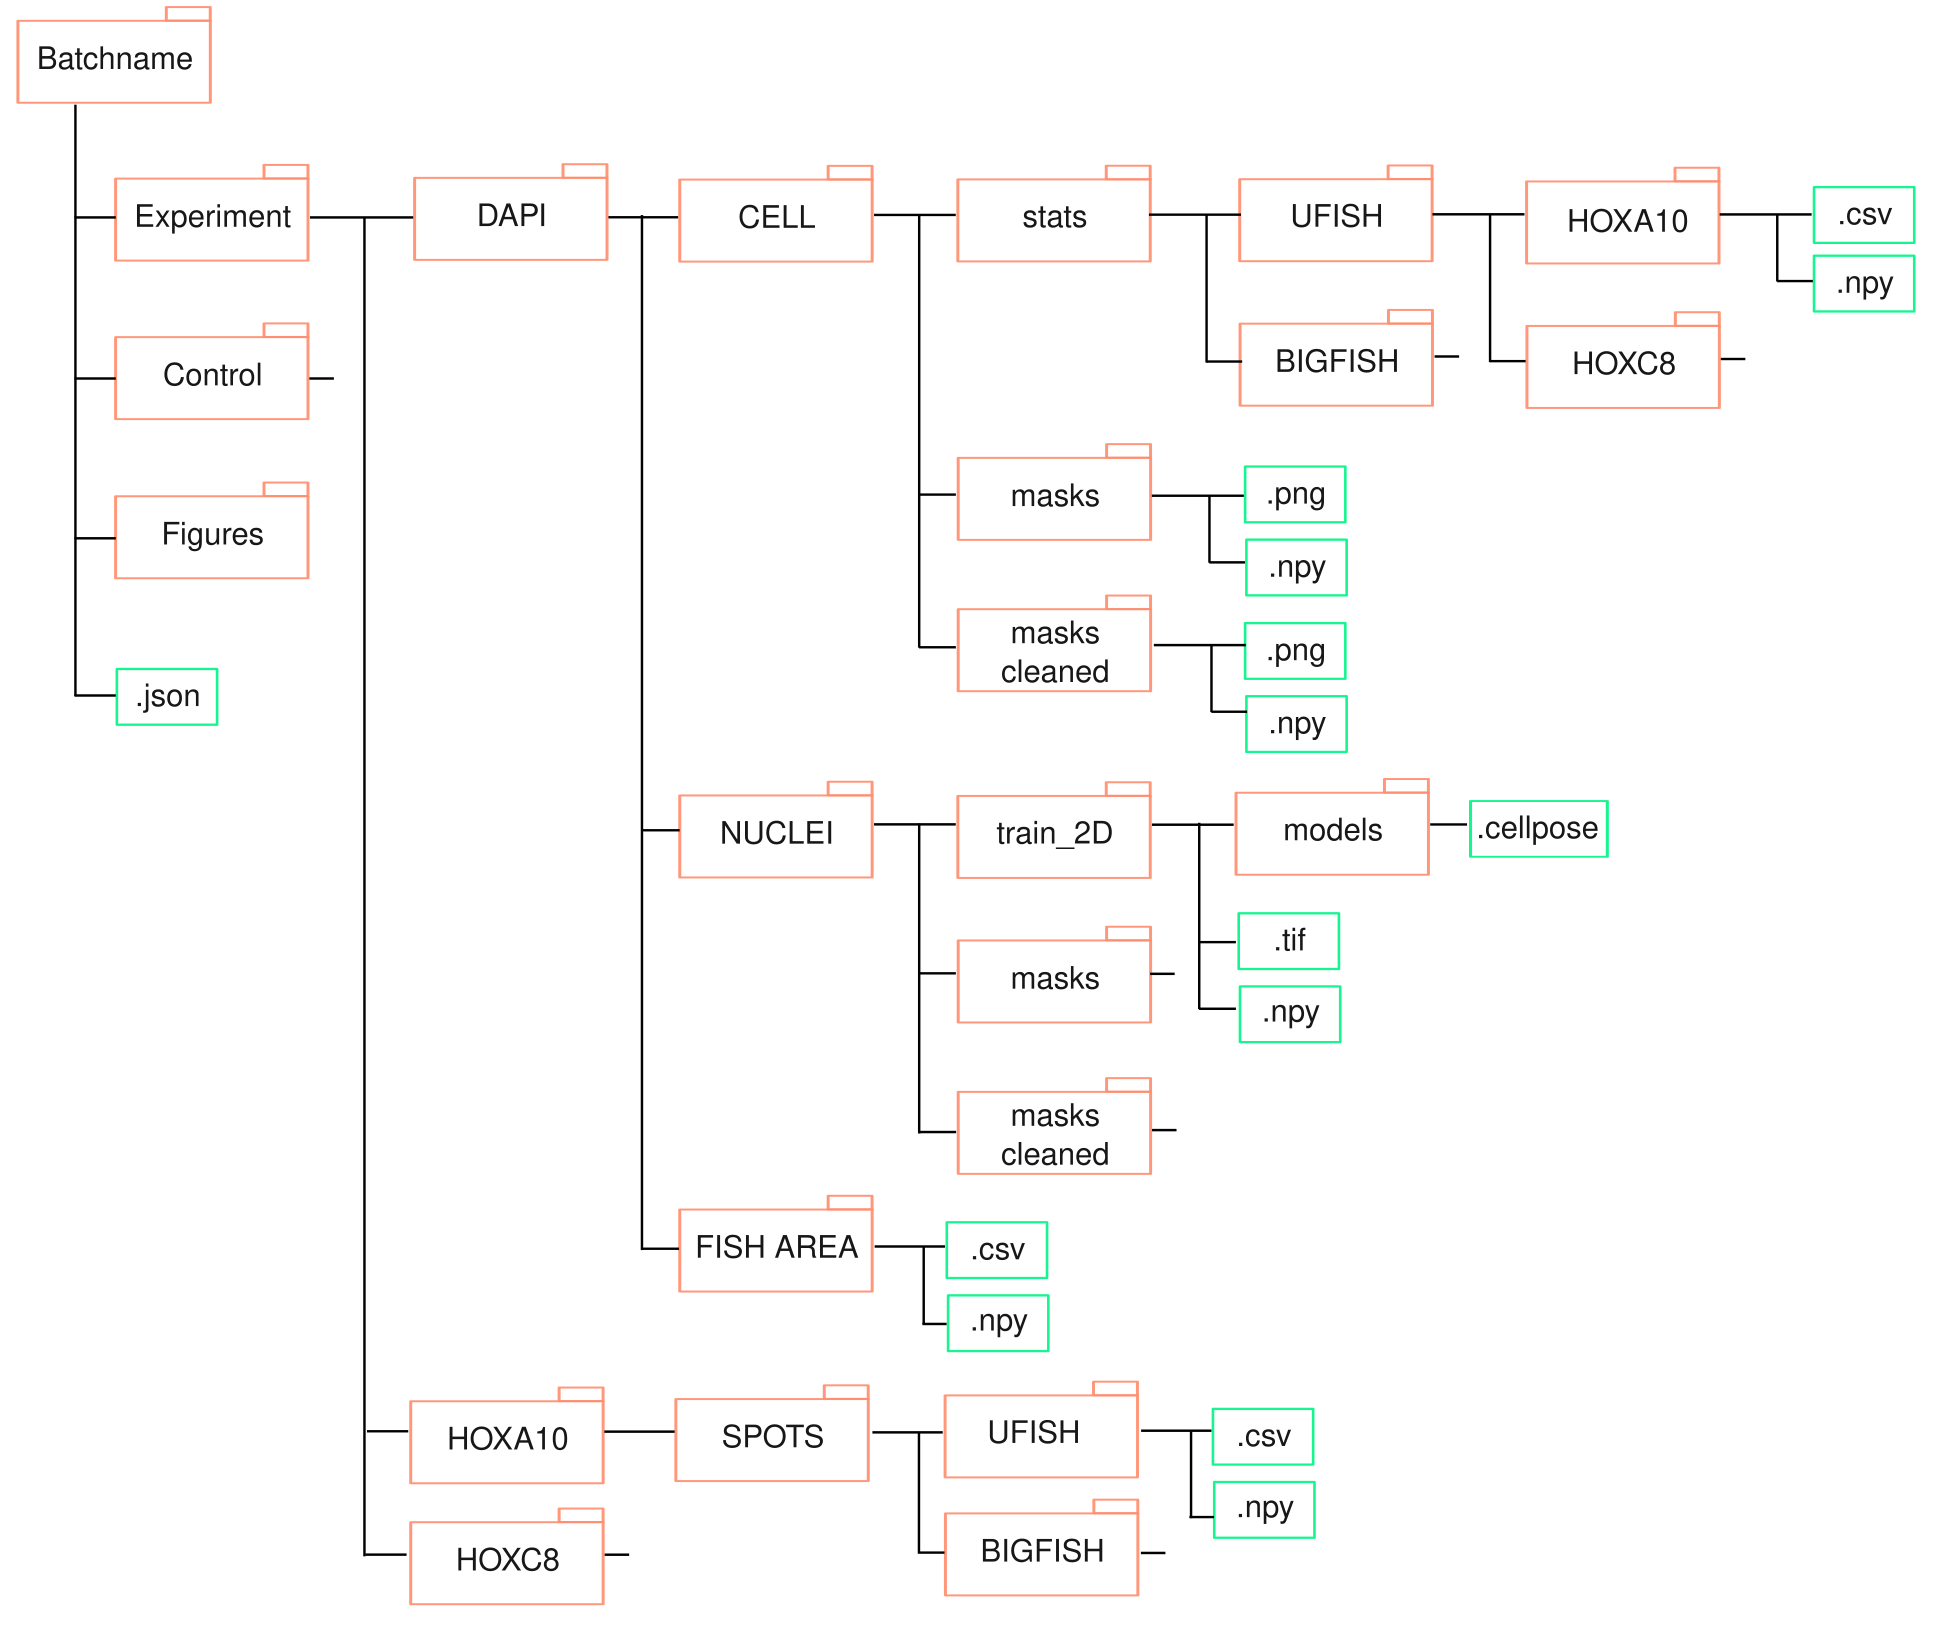
\includegraphics[width=1\textwidth]{Folder_struct.png} % Adjust width as needed
  \caption{Folder structure of the pipeline.}
  \label{fig:my_image} % For referencing the figure later
\end{figure}
 
  \newpage


       The project starts with two folders placed side to side : HOX pipeline and src. The src folder contains the main functions called in the pipeline. HOX pipeline contains three folders Acquisition, Analysis and Code. Code contains the jupyter notebooks that constitute the pipeline. In the folder Acquisition one can put the raw files, in the folder Analysis, we will put all the results (figures and intermediary files).

The arborescence of folders in Analysis is built as the execution of the pipeline progresses. We define, in the first notebook a batchname as a collection of experiments.  This batchname can for example be subdivided in what I call modalities, which are experiments conditions, for instance Experiment and Control. Each condition can be defined as a subset of experiments over which all the pipeline will run. Then, for each modality, I create a folder per channel : the DAPI, the HOXA10 and HOXC8. DAPI corresponds to the fluorescence coming from the nucleus (DAPI is a fluorescent molecule that binds to A and T nucleotides from the DNA). HOXA10 and HOXC8 corresponds to the channels that sense the fluorescence coming from that particular genes. 

In the DAPI folder there are three folders NUCLEI, CELL and $\text{FISH\_AREA}$. In nuclei, when the images are 2D, we directly copy them into the folder $\text{NUCLEI/train\_2D}$.  When images are 3D, we do a maxprojection of the original stack of images (in fact we do a subselection of the z’s at which the focus is better, and then we do a maxprojection). With these 2D images, we train a model in Cellpose. Cellpose stores the segmentation masks together with the images and creates a folder called models in which he stores the models.
In this pipeline in particular, as we can’t segment the cell bodies, we create artificially a mask dilating the cellpose masks, and store them in DAPI/CELL/masks. Nonetheless, for other cell types, in which we use cellmask for instance in the DAPI channel or just using a FISH channel, it is possible to segment the cellbody. That is why it is important to create a separate folder for each structure (cell and nuclei). For instance in the case in which we use cell mask, we copy the same 2D projected images of the DAPI channel into$\text{DAPI/CELL/train\_2D}$. and $\text{DAPI/NUCLEI/train\_2D}$.
In this way, the masks generated by cellpose won’t erase themselves, and the models will be unambiguously identified. 

This example aims at highlighting the complexity of creating a good folder structure that can adapt to every condition. There is another example of the same kind in our pipeline. When detecting spots, we might choose between two methods called BIGFISH and UFISH. For each gene therefore we have to create a folder  BIGFISH and a folder UFISH in which we will store the results. Now, when doing the single cell statistics, we don’t have to forget that there are two methods to detect spots on which the statistics rely. Therefore, we have to create folders stats/{method}/{gene}, where method = BIGFISH and UFISH and gene = HOXA10 and HOXC8.




\subsection{Quality control}

    As much as possible, in each processing step, we must be able to visualize the result of the processing on the raw data.  To this effect, I use napari viewers, that allow to overlay images,  labels (masks) and points (spots). Therefore when considering the .csv of a given gene in a given condition, we can pick a given point and to check if it corresponds to a real spot on the raw image, if it is in the mask in the vicinity of cells, on which we accept spots, and if the algorithm classified it as a spot to exclude for further analysis (example Spot ID = 3) in the above table.


\section{Conclusion}

Doing a image processing pipeline is not a trivial task. The most important tasks before starting is identifying the kind of experiments that have to be industrialized, and a finite range of  possibilities of those kinds of experiments. Then we need to find the right computational blocks that allow to answer our biological questions. Then it it important to identify what code parts can be reused, and then creating a folder structure that allows to cope with all the use cases/ options of the pipeline. 



\bibliographystyle{unsrtnat}
\bibliography{references}


\end{document}







